% +--------------------------------------------------------------------+
% | Sample Chapter 3
% +--------------------------------------------------------------------+
\cleardoublepage
% +--------------------------------------------------------------------+
% | Replace "This is Chapter 3" below with the title of your chapter.
% | LaTeX will automatically number the chapters.
% +--------------------------------------------------------------------+
    %\renewcommand{\chaptername}{Part}
    %\renewcommand{\thechapter}{}
\chapter{Implementation}
\label{makereference}
\begin{minipage}{\textwidth}
\section{General overview of the system}
The camera provides the pixels in the image by bands. The first operations to be performed with this data are to calculate the average, with it the deviation and then the covariance. Because of the relative simplicity of these operations but their high memory requirements, these three operations are performed on a CPU and their results sent to the FPGA. The FPGA will start the calculation of the subsequent operations only when it has the complete results of the covariance.

The data calculated by the CPU is entered into the FPGA through FIFOs.

The FPGA will then calculate the inverse of the matrix. Meanwhile the CPU will have to write the calculated averages and the values it had previously received from the camera, one by one. When the inverse is finished, the FPGA will perform the last two matrix multiplications and save the resulting data. With the last pixel processed, the FPGA will write the anomalies ordered from highest to lowest in another FIFO to be read by the CPU.

\section{Description by module}
\subsection{Control}
This module acts on the lower modules, both to control the data transfer between them and to arbitrate the access to the RAMS and the FIFOs that communicate with the CPU.

It is worth mentioning that it also performs some checks in the covariance transfer to ensure that the first division of the inverse is not performed with a 0, that is, that the position (0, 0) in the covariance matrix is different from 0.
\end{minipage}
\setcounter{page}{20}

\begin{figure}
\centering\textbf{
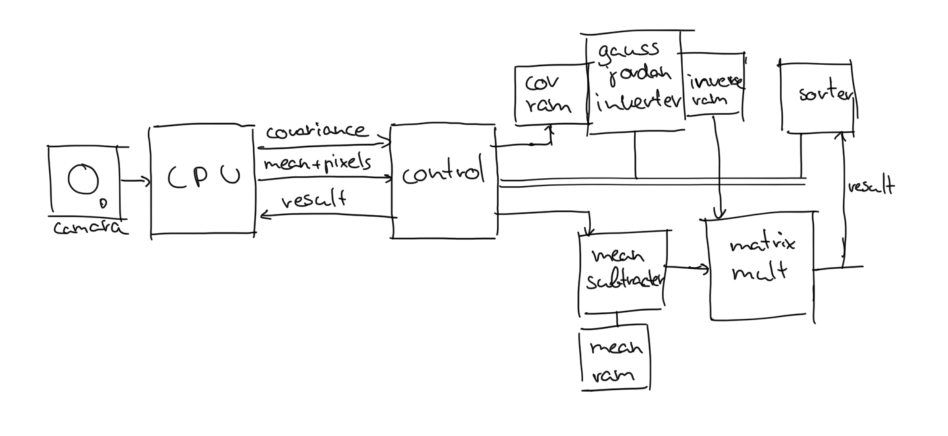
\includegraphics[height=7.5in]{figures/bus.png}}
\caption[A schematic of the top block]{A schematic of the whole system}
  \label{fig:bus}
\end{figure}

%\begin{lstlisting}
%IDLE:
%  if start then
%    goto READ
%
%READ:
%  while(fifo not empty)
%    read covariance row from fifo
%    if 0 then
%      swap
%    write covariance row to ram
%  if all rows written
%    goto INVERSE
%
%INVERSE:
%  start inverse
%  if inverse finished
%    goto MEAN SUBTRACTION
%
%MEAN SUBTRACTION:
%  start mean subtraction
%  if first result ready
%    goto MATRIX MULTIPLICATION
%
%MATRIX MULTIPLICATION:
%  start matrix multiplication
%  if first result ready
%    goto SORTER
%
%SORTER:
%  start SORTER
%  if matrix multiplication finished
%    write sorter results
%\end{lstlisting}
%
%
%\begin{figure}[h!]
%\centering
%\includegraphics[height=8in]{figures/flowchart.png}
%\caption{Tengo que elegir como lo prefiero}
%  \label{fig:ventana}
%\end{figure}
%\clearpage

\subsection{Inverter}
The inverse is the most complex module and the one that consumes more hardware resources. In addition, the study carried out on software has shown that it is by far the step most susceptible to worsening the accuracy of the final results. For these reasons, special emphasis has been placed on its design.

\begin{figure}[h!]
\centering\textbf{
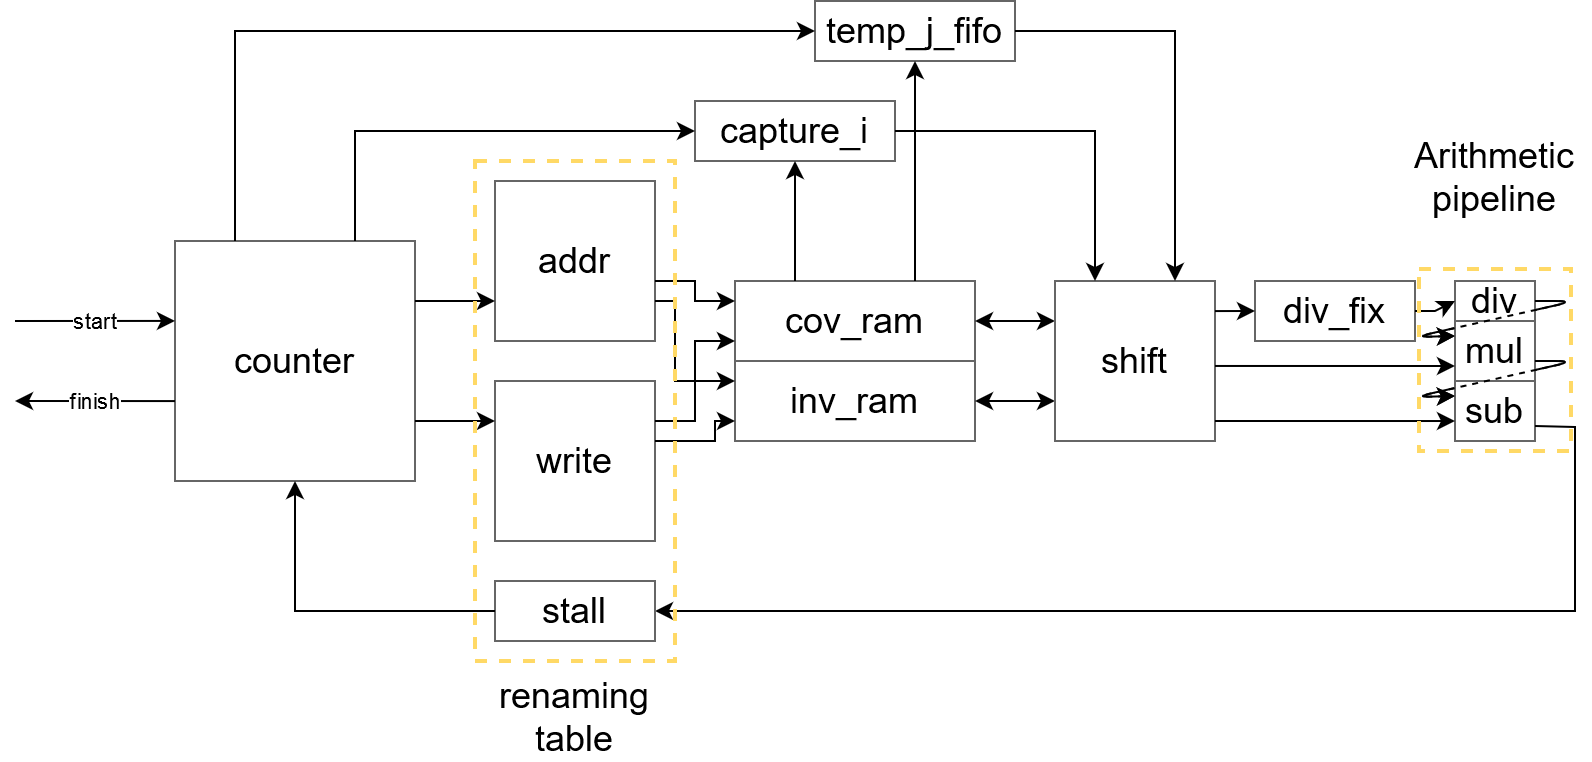
\includegraphics[height=2.5in]{figures/gauss.png}}
\caption{Schematic of the implemented inverter}
  \label{fig:gauss}
\end{figure}

As can be seen in \autoref{fig:gauss}, there are numerous processes and sub-modules within the inverter. The process that acts as an interface to the outside is \textit{counter}, which as its name suggests contains counters to calculate the rows to be read, written, etc. It is the main process of the module. The counters are translated into addresses by another pair of processes, more specifically \textit{addr}, \textit{write} and \textit{stall} and a renaming table to which these three have access. The data that are read from the memories are then saved in temporary storage or directly to the arithmetic units. Before the arithmetic units is another process, \textit{shift}, which shifts the data as modeled in software. These units are used for the three steps of the algorithm, upper triangle, lower triangle and diagonal, and it is the \textit{counter} process that controls their execution order. The rest of the processes will be explained in more detail within the chapter.

\pagebreak
\subsubsection{Agorithm optimizations for hardware}
To improve the performance of the module, operations on the $A$ matrix and the $A{-1}$ matrix are executed simultaneously. In addition, the divisor and DSP pipelines are used to queue all possible consecutive operations. Pipeline stalling only occurs, if calculations are still being processed with the last pivot row.
\autoref{latencias} shows the arithmetic units inside the module and their latencies. These latencies represent the length of its pipeline.
\newcommand{\hr}[1]{%
  \colorbox{red!20}{$\displaystyle#1$}}
\newcommand{\hg}[1]{%
  \colorbox{green!20}{$\displaystyle#1$}}
\newcommand{\hb}[1]{%
  \colorbox{blue!20}{$\displaystyle#1$}}
\begin{table}[h!]
\begin{center}
 \begin{tabular}{|c c c c|} 
 \hline
 Arithmetic Unit & Latency & Quantity & Remarks\\ [0.5ex] 
 \hline\hline
 \hr{Division} & 77 & 1 & Only one division is required each cycle \\ 
 \hline
 \hg{Multiplication} & 6 & bands*2 & To compute a whole row for both $A$ and $A^-1$ \\
 \hline
 \hb{Subtraction} & 2 & bands*2 & To compute a whole row for both $A$ and $A^-1$ \\
 \hline
\end{tabular}
\end{center}
\caption[Latencies for some arithmetic units]{Latencies and number of the arithmetic units in the inverter module.}
\label{latencias}
\end{table}

Equations \ref{pip_pop} indicate which calculations are found within the DSP pipeline at any given time. The results of each operation are sent directly to the calculation of the next operation, while the counters control that the other operands arrive at the right time.

\newcommand{\twodots}{\MTFlushSpaceAbove\vdotswithin{\gets}&&\vdotswithin{\gets}\MTFlushSpaceBelow}
\begin{figure}[h!]
\begin{align*}
%A^{-1}[87]\gets&A^{-1}[87]-A[i]^{-1}*A[87][i]/A[i][i],\ 
%&A[87]\gets&A[87]-A[i]*A[\jv][i]/A[i][i]\\
%\twodots
A^{-1}[86]\gets&A^{-1}[86]-A[i]^{-1}*\hr{A[86][i]/A[i][i]},\ 
&A[86]\gets&A[86]-A[i]*A[86][i]/A[i][i]\\
\twodots
A^{-1}[10]\gets&A^{-1}[10]-A[i]^{-1}*\hr{A[10][i]/A[i][i]},\ 
&A[10]\gets&A[10]-A[i]*A[10][i]/A[i][i]\\
A^{-1}[9]\gets&A^{-1}[9]-\hg{A[i]^{-1}*div\_result},\ 
&A[9]\gets&A[9]-\hg{A[i]*div\_result}\\
\twodots
A^{-1}[3]\gets&A^{-1}[3]-\hg{A[i]^{-1}*div\_result},\ 
&A[3]\gets&A[3]-\hg{A[i]*div\_result}\\
A^{-1}[2]\gets&\hb{A^{-1}[2]-mul\_result},\ 
&A[2]\gets&\hb{A[2]-mul\_result}\\
A^{-1}[1]\gets&\hb{A^{-1}[1]-mul\_result},\ 
&A[1]\gets&\hb{A[1]-mul\_result}\\
A^{-1}[0]\gets&\hb{sub\_result},\ 
&A[0]\gets&\hb{sub\_result}
\end{align*}
\caption[Arithmetic pipeline]{Operations representing the arithmetic pipeline at any given moment. Colors denote if a operation is currently in progress.}
\label{pip_pop}
\end{figure}

\pagebreak
One of the operands is the row \j, which is used at two different times within the algorithm (see \autoref{jjj}). Since a second read on the BRAM cannot be done since it is busy performing the read of the next operations, this data is stored at the time of reading in a FIFO and will be fetched when needed.
\newcommand{\highlight}[1]{%
  \colorbox{yellow!20}{$\displaystyle#1$}}
\begin{figure}[h!]
\[A^{-1}[j] \gets \highlight{A^{-1}[j]}-A[i]*\highlight{A[j][i]}/A[i][i]\]
\caption[Data depency in the pipeline]{As can be seen in the algorithm, row j is used at two different times.}
\label{jjj}
\end{figure}
\\
\\
Additionaly, it can be observed that in the first step in which the upper triangular matrix is constructed, the algorithm requires a check on the pivot row and a possible exchange of rows. This is necessary because this value is later the dividend, so a 0 would cause a failure in the calculation.
\\
BRAM memory readings have a latency cycle, so reading an inappropriate value two cycles in a row -in the case of reading an inappropriate and then an appropriate value, there would be the possibility of performing an inplace row swap with the pivot and the row just after it- would not only add latency to the calculation but also increase the complexity of the module. Therefore, the dividend checks are done on the writes, recorded in a renaming table that will be checked at the time of reading. This ensures that the reads will always be valid for the calculation. In the case of the very first division, this dividend comes directly from the CPU and the upper module \textit{control} is responsible for reordering this row if necessary.
\\
This renaming table is located in registers, so it is possible to access it without any latency and as it only contains indexes, it does not overload the FPGA resources. In addition, this table is local, so the results have to be reordered in the RAM itself before leaving the inverse module. Since these swaps only occur in the calculation of the upper triangle, the lower triangle can be used to reorder them. The reordering system is very simple, the data enters the pipeline according to the order that exists in the renaming table and is written in its natural order. This implies that the results of this reordering will be correct as long as both rows that have been rotated are at the same time in the processing pipeline, which in the case of fixed point is approximately 90 in size. Experimental results show that it is rarely necessary to rotate rows -although enough to recommend the inclusion of a method to deal with it-, and that these rotations rarely exceed one or two positions in the pipeline.
\\
\\
In the transformation to integer arithmetic it was discovered that the calculation of the inverse is the one introducing more error in the final results of the algorithm, therefore an exhaustive study on how to minimize it has been made. For this it has been necessary to reduce the values in which the limited precision produced overflows and increase small values to give them more weight in the operations. By performing the operations of identity generation, upper triangle, lower triangle and diagonal independently, it has been possible to place different shift values and further refine the resolution of the algorithm. These operations are performed by the \textit{shift} process.
\\
It should also be said that there is an error in the generation of Xilinx dividers. When you enter numbers near the precision limit you lose control of the sign. Therefore, \textit{div\_fix}, a process that converts all the entered operands into positives and saves their position in a pipeline has been placed before the division. When the results are produced, the tag is checked in the pipeline, the negative is calculated and replaced if necessary.

\subsection{Mean subtract}

\begin{figure}[h!]
\centering\textbf{
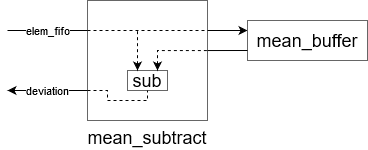
\includegraphics[height=1.5in]{figures/subtract.png}}
\caption{Schematic of mean subtract.}
  \label{fig:subtract}
\end{figure}
The \textit{mean subtract} module receives the calculated average and the original pixels of the image and subtracts them. This calculation is the deviation and although it had already been calculated by the CPU, it is possible that the latter discards the data to free up space. The calculation of the average is required because it is assumed that its size being much smaller, the CPU can keep it in memory. In case the deviation can be received directly from the CPU, this module can be simply deleted.
The module receives the elements from the upper module that reads them from the same FIFO. The first elements are the average and are stored in a BRAM that is treated as a circular buffer, and the following elements are directly subtracted and returned to the upper module again.


\subsection{Matrix multiplication}


\newcommand\rb{\colorbox{red!20}}
\newcommand\bb{\colorbox{blue!20}}
\newcommand\gb{\colorbox{green!20}}
\newcommand\rr{\rowcolor{red!20}}
\newcommand\br{\rowcolor{blue!20}}
\newcommand\gr{\rowcolor{green!20}}
As noted above (see \ref{alternativa}), this calculation can be implemented in two different ways.
\noindent Following will be a comparison of the first required multiplication in both methods:
\begin{quote}
	\((x-\mu)^{T} K^{-1}_{N \times N}\):	
	A row from the inverse and the whole column of the deviation get read, each element multiplied with its correspondent and all products added together. If stalls were to be avoided, this sum would need to be computed every cycle, which can easily be achieved with an adder tree.
\end{quote}

\begin{figure}[h]%t=top, b=bottom, h=here
\[
\begin{pmatrix}
\rr a & b & c \\ 
\br d & e & f \\ 
\gr g & h & i
\end{pmatrix}
*
\begin{pmatrix}
1\\
2\\
3
\end{pmatrix}
=
\begin{pmatrix}
\rr 1*a+2*b+3*c\\
\br 1*d+2*e+3*f\\
\gr 1*g+2*h+3*i
\end{pmatrix} 
\]
\caption[First proposed method for the matrix multiplication]{First proposed method for the computation of a single pixel: red, blue and green represent data processed in the first, second and third cycles respectively. Note that the entire deviation data of that pixel gets used every cycle}
\end{figure}
		
\begin{quote}
	\(K^{-1}_{N \times N} (x-\mu)\):
	The inverse gets also read row by row, but the deviation matrix only by elements. Each element of the first row of the matrix gets multiplied with the first element of the deviation, the result accumulated, and continued with the next pair row/element. This goes for \(N\) cycles, that is, a whole inverse matrix and a whole pixel in the deviation matrix. The result is \(N\) accumulated values which get flushed every \(N\) cycles, which ends up being the same throughput as the former method.
\end{quote}

\begin{figure}[h]%t=top, b=bottom, h=here
\[
\begin{pmatrix}
\rb1 & \bb 2 & \gb 3
\end{pmatrix}
*
\begin{pmatrix}
\rr a & b & c \\ 
\br d & e & f \\ 
\gr g & h & i
\end{pmatrix}
=
\begin{pmatrix}
\rb{1*a}+\bb{2*d}+\gb{3*g} & \rb{1*b}+\bb{2*e}+\gb{3*h} & \rb{1*c}+\bb{2*f}+\gb{3*i}
\end{pmatrix} 
\]
\caption[Second proposed method for the matrix multiplication]{Second proposed method: red, blue and green represent data processed in the first, second and third cycles respectively. Here only an element of the deviation data gets accessed each cycle.}
\end{figure}

While both methods have equivalent cost in time -the former has the added latency of the adder tree, the latter the latency of the accumulators- and also similar cost in DSP usage, data input by row is less taxing on the CPU and its FIFO structure can be reused for the second multiplication. Henceforth, the second approach was chosen.


\begin{figure}[h!]
\centering\textbf{
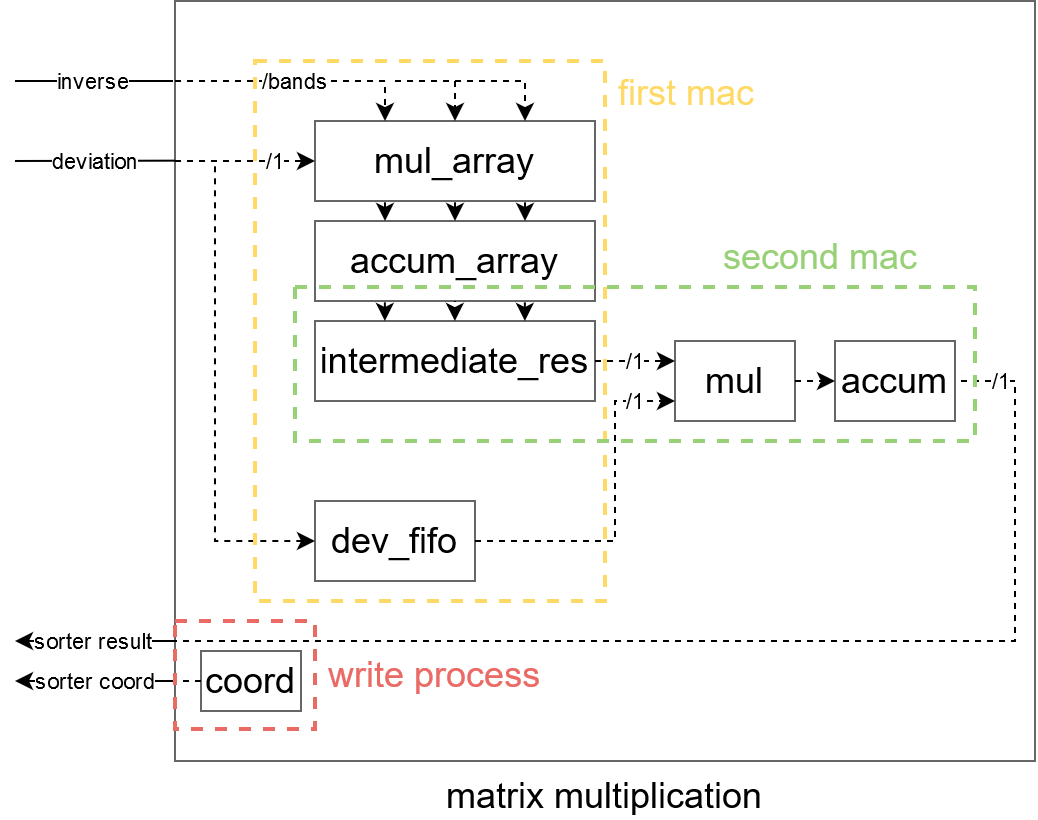
\includegraphics[height=3.5in]{figures/mult.png}}
\caption{Schematic of the dual matrix multiplier}
  \label{fig:mult}
\end{figure}

The second multiplication is similar in both steps, a \(1 \times N\) by \(N \times 1\) multiplication. One operand comes every cycle and each \(N\) cycles all products get added together. This sum is realized through an accumulator.\\

The module contains three subprocesses:
\begin{itemize}
	\item \emph{first\_mac} reads the inverse and performs its multiplication with the received deviation. This deviation is also stored in a FIFO. The products are then accumulated till a whole pixel has been computed.
	\item \emph{second\_mac} stores the results of \emph{first\_mac} in registers and performs the multiplication with data from the FIFO, with the result being accumulated. Every cycle, the registers are shifted so a new multiplication is done.
	\item \emph{write\_proc} controls the writing of the results from \emph{second\_mac} to the sorter and computes the coords.
\end{itemize}



\subsection{Coordinate sorter}
\begin{figure}[h!]
\centering\textbf{
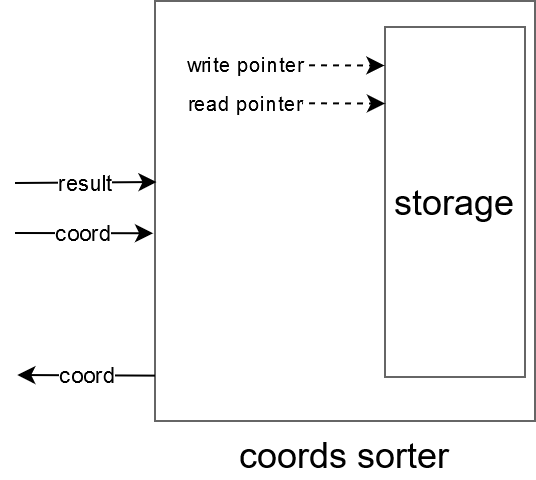
\includegraphics[height=2.5in]{figures/sort.png}}
\caption{Schematic of the coordinate sorter}
  \label{fig:sorter}
\end{figure}
This module receives a value and a pair of coordinates every \textit{bands} cycles. These values are written in a BRAM memory that acts as an ordered list. Each entered value is compared with the head of the list, the highest value is saved and the other is saved in a temporary variable, compared with the second value in the list, and so on. Since a value is received each \textit{bands}, the maximum number of possible values to be stored in this list is also \textit{bands}. The rest of the values are discarded. When the last value has been introduced, the module communicates the highest pixels, that is, the most anomalous ones, to the superior module so that they are communicated to the CPU.

